%-------------------------------------------------------------------------------
%-------------------------------------------------------------------------------
%-------------------------------------------------------------------------------
\chapter{Coefficients binomiaux (MP)}
%-------------------------------------------------------------------------------
%-------------------------------------------------------------------------------
%-------------------------------------------------------------------------------

Le but de ce problème est de définir les coefficients binomiaux et certaines de leurs utilisations. 

\medskip

{\bf Remarques}
\begin{itemize}
    \item Lorsque le résultat de la division de deux entiers doit être un entier on utilisera la division euclidienne : \Type{n // p}.

\item Lorsqu'un nombre d'opérations est demandé, il est possible de répondre sous la forme d'un grand ${\cal O}$.
\end{itemize}
%-------------------------------------------------------------------------------
%-------------------------------------------------------------------------------
%-------------------------------------------------------------------------------
\section{Calculs des coefficients binomiaux} 
%-------------------------------------------------------------------------------
%-------------------------------------------------------------------------------
%-------------------------------------------------------------------------------
\subsection{Calcul d'un coefficient} 
%-------------------------------------------------------------------------------
%-------------------------------------------------------------------------------
\begin{Exercise}
\it Écrire une fonction \type{facto(n)} qui calcule la factorielle de $n$.

Combien de multiplications l'appel de \type{facto(n)} effectue-t-il ?
\end{Exercise}
%-------------------------------------------------------------------------------
\begin{Answer}
\begin{lstlisting}
def facto(n):
    f = 1
    for k in range(1, n+1):
        f = f * k
    return f
\end{lstlisting}
Il y a $n$ multiplications.
\end{Answer}
%-------------------------------------------------------------------------------
%-------------------------------------------------------------------------------
\begin{Exercise}
\it En utilisant la définition $\displaystyle \binom np = \frac{n!}{p!(n-p)!}$ écrire une fonction \type{binom\_f(n, p)} qui calcule $\displaystyle \binom np$.

Combien de multiplications et divisions l'appel de \type{binom\_f(n, p)} effectue-t-il ?
\end{Exercise}
%-------------------------------------------------------------------------------
\begin{Answer}
\begin{lstlisting}
def binom_f(n, p):
    return facto(n)//facto(p)//(facto(n-p)
\end{lstlisting}
Il y a $n +p + n - p = 2n$ multiplications et deux divisions entières, c'est un ${\cal O}(n)$.
\end{Answer}
%-------------------------------------------------------------------------------
%-------------------------------------------------------------------------------
\begin{Exercise}[label = exo:prod]
\it Exprimer $\displaystyle \binom n{k+1}$ en fonction de  $\displaystyle \binom nk$ pour $0\le k < n$.

En déduire une fonction \type{binom\_p(n, p)} qui calcule $\displaystyle \binom np$ en effectuant $p$ multiplications et $p$ divisions {\bf entières}.
\end{Exercise}
%-------------------------------------------------------------------------------
\begin{Answer}
$\displaystyle  \binom n{k+1} = \frac{n-k}{k+1} \binom nk$
\begin{lstlisting}
def binom_p(n, p):
    b = 1
    for k in range(p):
        b = b * (n-k) // (k+1)
    return b
\end{lstlisting}
\end{Answer}
%-------------------------------------------------------------------------------
%-------------------------------------------------------------------------------
\begin{Exercise}
\it Pourquoi est-il indispensable d'utiliser la division euclidienne dans \type{binom\_f(n, p)} ?
\end{Exercise}
%-------------------------------------------------------------------------------
\begin{Answer}
Les factorielles créent des nombres qui peuvent être très grands, la division peut alors être impossible. 
\end{Answer}
%-------------------------------------------------------------------------------
\newpage
%-------------------------------------------------------------------------------
\subsection{Calcul des coefficients pour $n$ fixé} 
%-------------------------------------------------------------------------------
%-------------------------------------------------------------------------------
On aura besoin de tous les coefficients binomiaux de la forme $\binom n k$ pour un $n$ fixé ; on notera qu'il y en a $n+1$.

Par exemple \type{liste\_binom(8)} doit renvoyer \type{[1, 8, 28, 56, 70, 56, 28, 8, 1]}.
%-------------------------------------------------------------------------------
%-------------------------------------------------------------------------------
\begin{Exercise}
\it En utilisant la fonction \type{binom\_f}, écrire une fonction \type{liste\_binom1(n)} qui renvoie la liste des coefficient binomiaux. On ne cherchera pas à optimiser les calculs, c'est l'objet de la question suivante.

Combien de multiplications et de divisions sont effectuées lors de l'appel de \type{liste\_binom1(n)} ?
\end{Exercise}
%-------------------------------------------------------------------------------
\begin{Answer}
\begin{lstlisting}
def liste_binom1(n):
    coefs = [0]*(n+1)
    for p in range(n+1):
        coefs[p] = binom_f(n, p)
    return coefs
\end{lstlisting}

On fait $n+1$ fois $2n+2$ opérations, soit $2(n+1)^2 = {\cal O}(n^2)$.
\end{Answer}
%-------------------------------------------------------------------------------
%-------------------------------------------------------------------------------
\medskip

En fait on fait plusieurs fois les mêmes calculs de factorielles dans la fonction ci-dessus.
%-------------------------------------------------------------------------------
%-------------------------------------------------------------------------------
\begin{Exercise}
\it Écrire une fonction \type{liste\_binom2(n)} qui renvoie la liste des coefficient binomiaux en faisant un nombre de produits et de divisions entières qui soit un ${\cal O}(n)$.

On pourra commencer par créer une liste des $p!$ pour $0\le p \le n$ en ne faisant que $n$ multiplications.
\end{Exercise}
%-------------------------------------------------------------------------------
\begin{Answer}
\begin{lstlisting}
def liste_binom2(n):
    fact = [1]*(n+1)
    for p in range(1, n+1):
        fact[p] = fact[p-1]*p
    coefs = [0]*(n+1)
    for p in range(n+1):
        coefs[p] = fact[n] // fact[p] // fact[n-p]
    return coefs
\end{lstlisting}
\end{Answer}
%-------------------------------------------------------------------------------
%-------------------------------------------------------------------------------
\begin{Exercise}
\it En utilisant la formule de l'exercice \ref{exo:prod} mais sans utiliser \type{binom\_p}, écrire une fonction \type{liste\_binom3(n)} de complexité en ${\cal O}(n)$ qui calcule la liste des coefficient binomiaux.
\end{Exercise}
%-------------------------------------------------------------------------------
\begin{Answer}
\begin{lstlisting}
def liste_binom3(n):
    coefs = [1]*(n+1)
    for p in range(n):
        coefs[p+1] = coefs[p] * (n-p) // (p+1)
    return coefs
\end{lstlisting}
La fonction effectue $n$ multiplications et $n$ additions.
\end{Answer}
%-------------------------------------------------------------------------------
%-------------------------------------------------------------------------------
\subsection{Triangle de Pascal} 
%-------------------------------------------------------------------------------
%-------------------------------------------------------------------------------
On va ici calculer tous les coefficients binomiaux de la forme $\binom qp$ avec $0\le p \le q \le n$ pour un $n$ fixé.

\medskip

On peut utiliser les fonctions précédentes : on crée une liste de listes vides que l'on remplit avec les résultats de \type{liste\_binom}
\begin{lstlisting}
def pascal1(n):
    triangle = [[]]*(n+1)
    for q in range(n+1):
        triangle[q] = liste_binom3(q)
    return triangle
\end{lstlisting}

Par exemple \type{pascal1(4)} renvoie \type{[[1], [1, 1], [1, 2, 1], [1, 3, 3, 1], [1, 4, 6, 4, 1]]}.

Si \type{liste\_binom3(q)} effectue $q$ multiplications et $q$ divisions alors \type{pascal1(n)} demande $\frac{n(n+1)}2$ multiplications et autant de divisions.

On peut remplacer les multiplications et divisions en utilisant la formule 
\[\binom qp = \binom{q-1}{p-1} + \binom{q-1}{p}\hbox{ pour }1\le p < q \le n\]
%-------------------------------------------------------------------------------
%-------------------------------------------------------------------------------
\begin{Exercise}[label=exo:pascal]
\it Écrire une fonction \type{pascal(n)} qui renvoie le triangle de pascal comme ci-dessus en n'effectuant que des additions.
Combien d'additions sont nécessaires pour calculer \type{pascal(n)} ?
\end{Exercise}
%-------------------------------------------------------------------------------
\begin{Answer}
\begin{lstlisting}
def pascal(n):
    C = [[]]*(n+1)
    for q in range(n+1):
        C[q] = [1]*(q+1)
        for p in range(1, q):
            C[q][p] = C[q-1][p-1] + C[q-1][p]
    return C
\end{lstlisting}

La boucle d'indice $p$ effectue $q-1$ additions (pour $q\ge 2$) : il y a $\frac{n(n-1)}2$ additions. 
\end{Answer}
%-------------------------------------------------------------------------------
%-------------------------------------------------------------------------------
\begin{Exercise}
\it Comment utiliser \type{pascal(n)} pour calculer la liste des $\binom np$, $0\le p \le n$, $n$ fixé ?
\end{Exercise}
%-------------------------------------------------------------------------------
\begin{Answer}\type{pascal(n)[n]}
\end{Answer}
%-------------------------------------------------------------------------------
%-------------------------------------------------------------------------------
Cette méthode a un temps de calcul plus élevé mais peut être préférée car elle n'utilise que des additions.

Cependant elle demande beaucoup de place en mémoire ($\frac{(n+2)(n+1)}2$ valeurs).
%-------------------------------------------------------------------------------
%-------------------------------------------------------------------------------
\begin{Exercise}[difficulty=2]
\it Écrire une fonction \type{liste\_binom4(n)} qui calcule la liste des $\binom np$ pour $0\le p \le n$ en n'effectuant que des additions et en ne définissant qu'une seule liste de taille $n+1$. 

Le nombre d'additions est inchangé par rapport à l'exercice \ref{exo:pascal}.
\end{Exercise}
%-------------------------------------------------------------------------------
\begin{Answer}
L'idée est de remplacer le terme d'indice $p$ par la somme des termes d'indices $p$ et $p-1$ en décroissant de $q-1$ jusqu'a 1.
\begin{lstlisting}
def liste_binom4(n):
    coefs = [1]*(n+1)
    for q in range(2, n+1):
        for p in range(q-1, 0, -1):
            coefs[p] = coefs[p] +coefs[p-1]
    return coefs
\end{lstlisting}
\end{Answer}
%-------------------------------------------------------------------------------
\newpage
%-------------------------------------------------------------------------------
%-------------------------------------------------------------------------------
\section{Application}
%-------------------------------------------------------------------------------
%-------------------------------------------------------------------------------
%-------------------------------------------------------------------------------
\subsection{Polynômes de Bernstein}
%-------------------------------------------------------------------------------
%-------------------------------------------------------------------------------
%-------------------------------------------------------------------------------
Pour une fonction continue sur $[0;1]$ on définit la suite des polynômes de Bernstein $\bigl(B_n(f)\bigr)$ par

\[B_n(f)(x)=\sum_{k=0}^n \binom nk{\textstyle f\left(\frac kn\right)} x^k(1-x)^{n-k}\]

On peut démontrer que la suite $\bigl(B_n(f)\bigr)$  converge uniformément vers $f$ sur $[a;b]$.

On voit qu'il suffit de connaître les valeurs de $f$ aux $n+1$ points $\frac kn$ avec $0\le k \le n$, pour définir $B_n(f)$ sur tout l'intervalle : les polynômes de Bernstein sont utilisés pour tracé des courbes définies par $n+1$ points, les courbes de Bézier d'ordre $n$.

On suppose donnée une fonction
\begin{lstlisting}
def f(x):
    ....
    return y 
\end{lstlisting}
%-------------------------------------------------------------------------------
%-------------------------------------------------------------------------------
\begin{Exercise}
\it Écrire une fonction \type{bernstein(n, f, x)} qui renvoie la valeur de $B_n(f)(x)$.
\end{Exercise}
%-------------------------------------------------------------------------------
\begin{Answer}
\begin{lstlisting}
def bernstein(n, f, x):
    C = liste_binom3(n)
    y = 0
    for x in range(n+1):
        y = y + C[k]*f(k/n)*x**k*(1-x)**(n-k)
    return y
\end{lstlisting}
\end{Answer}
%-------------------------------------------------------------------------------
%-------------------------------------------------------------------------------
%-------------------------------------------------------------------------------
\subsection{Lissage}
%-------------------------------------------------------------------------------
%-------------------------------------------------------------------------------
%-------------------------------------------------------------------------------
Lors d'une expérimentation les données sont acquises automatiquement à des intervalles de temps constant et sont restituées sous la forme d'une liste \type{x\_exp} de taille $N$. 

Malheureusement les incertitudes dans la mesure sont inévitables et les valeurs calculées ont une part d'aléatoire.

On va essayer de lisser la suite des valeurs en remplaçant chacune par une moyenne pondérée des valeurs voisines.  On choisit un lissage de Gauss à l'ordre $p$ :
\[\widehat x_i = \left\{\begin{matrix}
\displaystyle \frac 1{2^{2p}}\sum_{j=-p}^{p}\binom {2p}{j+p} x_{i+j}&\hbox{ pour }p\le i \le N-1-p\\ 
x_i&\hbox{ pour } i<p\hbox{ ou } i\ge N-p\end{matrix}\right.\]

Par exemple, pour $N=4$ et $p = 1$, $[x_0,x_1,x_2,x_3]$ devient
$\bigl[x_0,\frac{x_0+2x_1+x_2}4,\frac{x_1+2x_2+x_3}4,x_3\bigr]$
%-------------------------------------------------------------------------------
\begin{figure}[ht]
\begin{center}
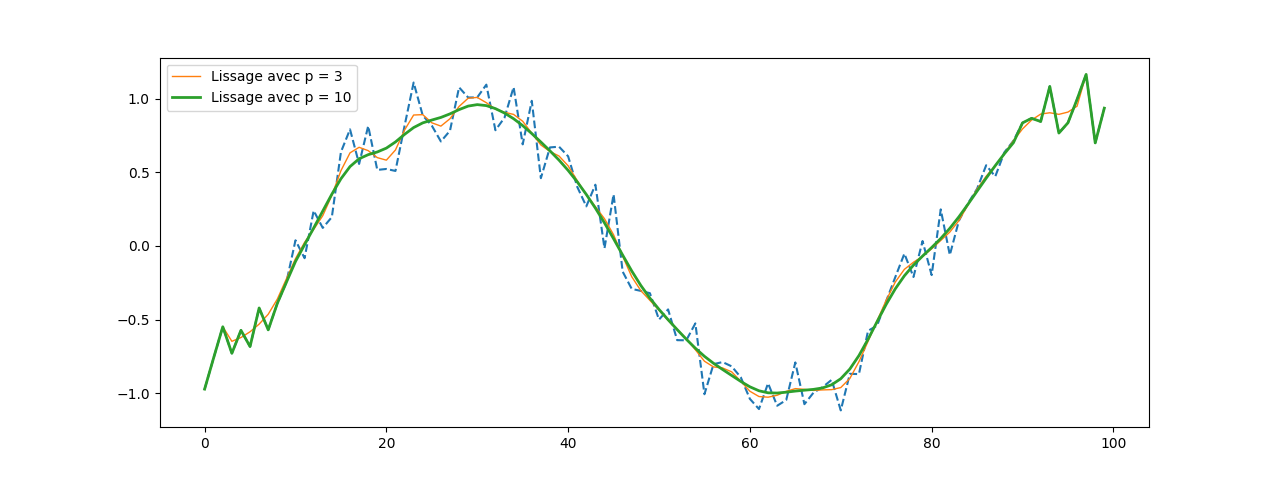
\includegraphics[width=\linewidth]{1MP_lissage}
\caption{Exemples de lissage, les valeurs aux bordx ne sont pas lissées}
\end{center}
\end{figure}
%-------------------------------------------------------------------------------
%-------------------------------------------------------------------------------
\begin{Exercise}  
\it Pourquoi divise-t-on par $2^{2p}$ ?
\end{Exercise}
%-------------------------------------------------------------------------------
\begin{Answer}
La somme des coefficients est $2^{2p}$.
\end{Answer}
%-------------------------------------------------------------------------------
%-------------------------------------------------------------------------------
\begin{Exercise}
\it On a fait le choix de ne pas modifier les $p$ premiers et les $p$ derniers termes : proposer une autre possibilité. Cette question n'a pas de réponse unique.
\end{Exercise}
%-------------------------------------------------------------------------------
\begin{Answer}On peut lisser en $i$ et en $n-i-1$ avec $2i+1$ points pour $0\le i < p$ :

$\displaystyle widehat x_i = \frac 1{2^{2i}}\sum_{j=0}^{2i}\binom {2i}{j} x_{j}$ et
$\displaystyle widehat x_{n-1-i} = \frac 1{2^{2i}}\sum_{j=n-1-2i}^{n-1}\binom {2i}{n-1-j} x_{j}$ et
\end{Answer}
%-------------------------------------------------------------------------------
%-------------------------------------------------------------------------------
\begin{Exercise}
\it Écrire une fonction \type{lissage(x, p)} qui renvoie la nouvelle liste des valeurs lissées obtenues à partie de la liste \type{x} en appliquant le lissage de Gauss à l'ordre $p$.
\end{Exercise}
%-------------------------------------------------------------------------------
\begin{Answer}
\begin{lstlisting}
def lissage(x, p):
    n = len(x)
    liss = [0]*n
    coefs = liste_binom3(n)
    for i in range(n):
        if i >= p and i < n - p:
            for j in range(i-p, i+p+1):
                liss[i] = liss[i] + x[j]*coefs[j-i+p]
        else:
            liss[i] = x[i]
    return liss
\end{lstlisting}
\end{Answer}
%-------------------------------------------------------------------------------
%-------------------------------------------------------------------------------
\begin{Exercise}
\it Quelle est la complexité de cette fonction ?
\end{Exercise}
%-------------------------------------------------------------------------------
\begin{Answer}

On compte le nombre d'additions et de multiplications : on en fait 
$(n-2p)2(2p+1)$
\end{Answer}
%-------------------------------------------------------------------------------
%-------------------------------------------------------------------------------
%-------------------------------------------------------------------------------
% %-------------------------------------------------------------------------------
% \begin{Exercise}
% \it 
% \end{Exercise}
% %-------------------------------------------------------------------------------
% \begin{Answer}
% \begin{lstlisting}
% \end{lstlisting}
% \end{Answer}
% %-------------------------------------------------------------------------------
% %-------------------------------------------------------------------------------


% On remarque que le lissage n'apparaît pas dans les valeurs extrêmes.
% \end{center}

% \newpage

% \section{Application 2 : polynômes de Bernstein}

% Pour une fonction continue sur $[0;1]$ on définit la suite des polynômes de Bernstein.\footnote{
% Il est a noter qu'en général $B_n(f)\left(\frac kn\right)$ n'est pas égal à $f\left(\frac kn\right)$ mais l'écart peut être rendu aussi petit que l'on veut pour $n$ assez grand.}, $\bigl(B_n(f)\bigr)_{n\in \N}$, par
% $\displaystyle B_n(f)(x)=\sum_{k=0}^n \binom nk{\textstyle f\left(\frac kn\right)} x^k(1-x)^{n-k}$.

% 

% \subsection{Cas d'une fonction}

% On suppose donnée une fonction
% \begin{lstlisting}
% def f(x):
%     ....
%     return y 
% \end{lstlisting}

% \begin{Exercise}
% \textit{\'Ecrire une fonction \type{bernstein(n,f,x)} qui renvoie la valeur de $B_n(f)(x)$.
% }
% \end{Exercise}
% \subsection{Cas d'une liste de valeurs}

% Comme signalé ci-dessus il suffit de connaître les valeurs d'une fonction en $n+1$ points pour déterminer les polynômes de Bernstein.

% On suppose fixées $n+1$ valeurs sous la forme d'une liste \type{c}.

% Toutes les fonctions $f$ telles que $f\left(\frac kn\right) = c[k]$ définissent le même polynôme de Bernstein $B_n(f)$ : on le notera $B_n(c)$.

% \begin{Exercise}
% \textit{\'Ecrire une fonction \type{bezier(c,x)} qui renvoie la valeur de $B_n(c)(x)$ où $c$ est une suite de longueur $n+1$.}
% \end{Exercise}

% \begin{Exercise}
% \textit{Combien de multiplications sont nécessaires pour calculer  \type{bezier(c,x)} ?\\
% On considèrera que l'exponentiation \type{x**k} demande $k-1$ multiplications.}
% \end{Exercise}

% \begin{center}
% \includegraphics[width=0.5\linewidth]{5.png}

% Courbe de Bézier d'ordre 7 et ses points de contrôle.
% \end{center}

% $x(t)$ et $y(t)$ sont les fonctions \type{bezier(cx,t)} et \type{bezier(cy,t)} où \type{cx} et \type{cy} sont les listes des abscisses et des ordonnées des points.
